\documentclass{article}\usepackage[]{graphicx}\usepackage[]{color}
%% maxwidth is the original width if it is less than linewidth
%% otherwise use linewidth (to make sure the graphics do not exceed the margin)
\makeatletter
\def\maxwidth{ %
  \ifdim\Gin@nat@width>\linewidth
    \linewidth
  \else
    \Gin@nat@width
  \fi
}
\makeatother

\definecolor{fgcolor}{rgb}{0.345, 0.345, 0.345}
\newcommand{\hlnum}[1]{\textcolor[rgb]{0.686,0.059,0.569}{#1}}%
\newcommand{\hlstr}[1]{\textcolor[rgb]{0.192,0.494,0.8}{#1}}%
\newcommand{\hlcom}[1]{\textcolor[rgb]{0.678,0.584,0.686}{\textit{#1}}}%
\newcommand{\hlopt}[1]{\textcolor[rgb]{0,0,0}{#1}}%
\newcommand{\hlstd}[1]{\textcolor[rgb]{0.345,0.345,0.345}{#1}}%
\newcommand{\hlkwa}[1]{\textcolor[rgb]{0.161,0.373,0.58}{\textbf{#1}}}%
\newcommand{\hlkwb}[1]{\textcolor[rgb]{0.69,0.353,0.396}{#1}}%
\newcommand{\hlkwc}[1]{\textcolor[rgb]{0.333,0.667,0.333}{#1}}%
\newcommand{\hlkwd}[1]{\textcolor[rgb]{0.737,0.353,0.396}{\textbf{#1}}}%
\let\hlipl\hlkwb

\usepackage{framed}
\makeatletter
\newenvironment{kframe}{%
 \def\at@end@of@kframe{}%
 \ifinner\ifhmode%
  \def\at@end@of@kframe{\end{minipage}}%
  \begin{minipage}{\columnwidth}%
 \fi\fi%
 \def\FrameCommand##1{\hskip\@totalleftmargin \hskip-\fboxsep
 \colorbox{shadecolor}{##1}\hskip-\fboxsep
     % There is no \\@totalrightmargin, so:
     \hskip-\linewidth \hskip-\@totalleftmargin \hskip\columnwidth}%
 \MakeFramed {\advance\hsize-\width
   \@totalleftmargin\z@ \linewidth\hsize
   \@setminipage}}%
 {\par\unskip\endMakeFramed%
 \at@end@of@kframe}
\makeatother

\definecolor{shadecolor}{rgb}{.97, .97, .97}
\definecolor{messagecolor}{rgb}{0, 0, 0}
\definecolor{warningcolor}{rgb}{1, 0, 1}
\definecolor{errorcolor}{rgb}{1, 0, 0}
\newenvironment{knitrout}{}{} % an empty environment to be redefined in TeX

\usepackage{alltt}

% \usepackage[utf8]{inputenc}
\usepackage{amsmath}
\usepackage{fancyhdr}
\usepackage{array}
\usepackage{longtable}
\usepackage{graphicx}
\usepackage{color}
\usepackage[letterpaper, margin=1in]{geometry}
\usepackage{lscape}
\newcommand{\blandscape}{\begin{landscape}}
\newcommand{\elandscape}{\end{landscape}}
\usepackage{dcolumn}
\usepackage{bbm}
\usepackage{threeparttable}
\usepackage{booktabs}
\usepackage{expex}
\usepackage{pdflscape}
\usepackage{rotating, graphicx}
\usepackage{tabulary}
\usepackage{lscape}
\usepackage{makecell}
\usepackage{algorithm}
\usepackage{multirow}
\usepackage{colortbl}
\usepackage{longtable}
\usepackage{array}
\usepackage{multirow}
\usepackage{wrapfig}
\usepackage{float}
\usepackage{pdflscape}
\usepackage{tabu}
\usepackage{threeparttable}

\title{%
Homework 3\\
\large Applied Mutlivariate Analysis}
\date{September 22, 2018}
\author{Emorie Beck}
\IfFileExists{upquote.sty}{\usepackage{upquote}}{}
\begin{document}
\maketitle
% \SweaveOpts{concordance=TRUE}

\section{Workspace}
\subsection{Packages}



\begin{knitrout}
\definecolor{shadecolor}{rgb}{0.969, 0.969, 0.969}\color{fgcolor}\begin{kframe}
\begin{alltt}
\hlkwd{library}\hlstd{(car)}
\hlkwd{library}\hlstd{(knitr)}
\hlkwd{library}\hlstd{(psych)}
\hlkwd{library}\hlstd{(kableExtra)}
\hlkwd{library}\hlstd{(multcomp)}
\hlkwd{library}\hlstd{(lme4)}
\hlkwd{library}\hlstd{(plyr)}
\hlkwd{library}\hlstd{(tidyverse)}
\hlkwd{library}\hlstd{(MVN)}
\end{alltt}
\end{kframe}
\end{knitrout}



\subsection{data}
The file, Set\_5.csv, contains data from a study in which college students completed the NEO-PI Personality Inventory. This 240-item scale purportedly measures the Big Five personality dimensions, assumed to be fairly independent. The inventory is scored on 6 subscales per dimension, listed below. The file contains the subscale scores, rather than the individual items, which should help reduce the impact of the small sample size.\\

Neuroticism: Anxiety
Neuroticism: Angry\_Hostility
Neuroticism: Depression
Neuroticism: Self\_Consciousness
Neuroticism: Impulsiveness
Neuroticism: Vulnerability
Extraversion: Warmth
Extraversion: Gregariousness
Extraversion: Assertiveness
Extraversion: Activity
Extraversion: Excitement\_Seeking
Extraversion: Positive\_Emotions
Openness: Fantasy
Openness: Aesthetics
Openness: Feelings
Openness: Actions
Openness: Ideas
Openness: Values
Agreeableness: Trust
Agreeableness: Straightforwardness 
Agreeableness: Altruism
Agreeableness: Compliance
Agreeableness: Modesty
Agreeableness: Tender\_Mindedness
Conscientiousness: Competence
Conscientiousness: Order
Conscientiousness: Dutifulness
Conscientiousness: Achievement\_Striving: 
Conscientiousness: Self\_Discipline
Conscientiousness: Deliberation

\begin{knitrout}
\definecolor{shadecolor}{rgb}{0.969, 0.969, 0.969}\color{fgcolor}\begin{kframe}
\begin{alltt}
\hlstd{wd} \hlkwb{<-} \hlstr{"https://github.com/emoriebeck/homeworks/raw/master/multivariate/homeworks/homework5"}

\hlstd{dat} \hlkwb{<-} \hlkwd{sprintf}\hlstd{(}\hlstr{"%s/Set_5(2).csv"}\hlstd{, wd)} \hlopt
  \hlkwd{read.csv}\hlstd{(.,} \hlkwc{stringsAsFactors} \hlstd{= F)}

\hlkwd{head}\hlstd{(dat)}
\end{alltt}
\begin{verbatim}
##   ID Anxiety Angry_Hostility Depression Self_Consciousness Impulsiveness
## 1  2   2.625           2.000      1.750           2.250000         2.625
## 2  3   3.625           2.875      3.000           3.500000         4.250
## 3  4   3.000           2.750      2.625           2.875000         3.000
## 4  5   4.375           3.125      4.500           4.000000         3.875
## 5  6   3.500           2.875      3.000           2.571429         3.625
## 6  7   4.000           4.125      2.875           2.375000         4.000
##   Vulnerability   Warmth Gregariousness Assertiveness Activity
## 1      2.166667 4.666667          4.000      3.000000 4.833333
## 2      2.125000 4.500000          2.750      2.625000 3.000000
## 3      2.875000 3.750000          3.125      2.375000 3.250000
## 4      3.750000 3.250000          2.250      2.500000 1.875000
## 5      2.750000 3.750000          3.125      3.285714 3.500000
## 6      3.125000 3.500000          2.625      3.375000 3.125000
##   Excitement_Seeking Positive_Emotions  Fantasy Aesthetics Feelings
## 1              3.500             4.750 3.857143   3.571429 4.666667
## 2              2.875             3.500 3.500000   4.125000 3.625000
## 3              3.875             3.375 3.375000   3.500000 3.250000
## 4              2.750             2.625 3.000000   3.750000 4.250000
## 5              3.750             3.625 3.125000   1.625000 3.125000
## 6              2.000             3.375 3.500000   2.000000 3.250000
##    Actions Ideas Values Trust Straightforwardness Altruism Compliance
## 1 2.571429 4.400  4.600 5.000            2.166667 4.833333      2.750
## 2 3.000000 3.875  3.125 3.250            3.750000 3.625000      3.125
## 3 2.375000 4.125  3.500 3.250            3.125000 4.000000      3.750
## 4 3.375000 2.750  4.125 3.000            3.428571 3.875000      4.000
## 5 2.750000 2.500  3.625 3.375            3.250000 4.125000      3.625
## 6 2.625000 1.125  3.625 2.500            2.875000 3.000000      2.250
##   Modesty Tender_Mindedness Competence Order Dutifulness
## 1   4.000          3.833333       4.50 3.625    3.285714
## 2   2.625          3.250000       3.00 2.250    3.875000
## 3   2.750          3.250000       3.75 3.250    3.750000
## 4   4.125          3.750000       2.75 3.000    2.875000
## 5   3.375          3.375000       3.75 4.000    3.750000
## 6   2.625          3.375000       3.00 3.625    2.625000
##   Achievement_Striving Self_Discipline Deliberation
## 1             4.333333           4.250        2.875
## 2             2.750000           3.750        3.500
## 3             3.375000           3.375        3.125
## 4             2.875000           2.625        3.250
## 5             3.375000           2.875        3.375
## 6             3.000000           2.625        2.625
\end{verbatim}
\end{kframe}
\end{knitrout}

\begin{knitrout}
\definecolor{shadecolor}{rgb}{0.969, 0.969, 0.969}\color{fgcolor}\begin{kframe}
\begin{alltt}
\hlstd{source} \hlkwb{<-} \hlkwd{tribble}\hlstd{(}
\hlopt{~}\hlstd{Factor,} \hlopt{~}\hlstd{Facet,}
\hlstr{"Neuroticism"}\hlstd{,} \hlstr{"Anxiety"}\hlstd{,}
\hlstr{"Neuroticism"}\hlstd{,} \hlstr{"Angry_Hostility"}\hlstd{,}
\hlstr{"Neuroticism"}\hlstd{,} \hlstr{"Depression"}\hlstd{,}
\hlstr{"Neuroticism"}\hlstd{,} \hlstr{"Self_Consciousness"}\hlstd{,}
\hlstr{"Neuroticism"}\hlstd{,} \hlstr{"Impulsiveness"}\hlstd{,}
\hlstr{"Neuroticism"}\hlstd{,} \hlstr{"Vulnerability"}\hlstd{,}
\hlstr{"Extraversion"}\hlstd{,} \hlstr{"Warmth"}\hlstd{,}
\hlstr{"Extraversion"}\hlstd{,} \hlstr{"Gregariousness"}\hlstd{,}
\hlstr{"Extraversion"}\hlstd{,} \hlstr{"Assertiveness"}\hlstd{,}
\hlstr{"Extraversion"}\hlstd{,} \hlstr{"Activity"}\hlstd{,}
\hlstr{"Extraversion"}\hlstd{,} \hlstr{"Excitement_Seeking"}\hlstd{,}
\hlstr{"Extraversion"}\hlstd{,} \hlstr{"Positive_Emotions"}\hlstd{,}
\hlstr{"Openness"}\hlstd{,} \hlstr{"Fantasy"}\hlstd{,}
\hlstr{"Openness"}\hlstd{,} \hlstr{"Aesthetics"}\hlstd{,}
\hlstr{"Openness"}\hlstd{,} \hlstr{"Feelings"}\hlstd{,}
\hlstr{"Openness"}\hlstd{,} \hlstr{"Actions"}\hlstd{,}
\hlstr{"Openness"}\hlstd{,} \hlstr{"Ideas"}\hlstd{,}
\hlstr{"Openness"}\hlstd{,} \hlstr{"Values"}\hlstd{,}
\hlstr{"Agreeableness"}\hlstd{,} \hlstr{"Trust"}\hlstd{,}
\hlstr{"Agreeableness"}\hlstd{,} \hlstr{"Straightforwardness"} \hlstd{,}
\hlstr{"Agreeableness"}\hlstd{,} \hlstr{"Altruism"}\hlstd{,}
\hlstr{"Agreeableness"}\hlstd{,} \hlstr{"Compliance"}\hlstd{,}
\hlstr{"Agreeableness"}\hlstd{,} \hlstr{"Modesty"}\hlstd{,}
\hlstr{"Agreeableness"}\hlstd{,} \hlstr{"Tender_Mindedness"}\hlstd{,}
\hlstr{"Conscientiousness"}\hlstd{,} \hlstr{"Competence"}\hlstd{,}
\hlstr{"Conscientiousness"}\hlstd{,} \hlstr{"Order"}\hlstd{,}
\hlstr{"Conscientiousness"}\hlstd{,} \hlstr{"Dutifulness"}\hlstd{,}
\hlstr{"Conscientiousness"}\hlstd{,} \hlstr{"Achievement_Striving"}\hlstd{,}
\hlstr{"Conscientiousness"}\hlstd{,} \hlstr{"Self_Discipline"}\hlstd{,}
\hlstr{"Conscientiousness"}\hlstd{,} \hlstr{"Deliberation"}
\hlstd{)}

\hlstd{dat} \hlkwb{<-} \hlstd{dat} \hlopt \hlkwd{select}\hlstd{(ID, source}\hlopt{$}\hlstd{Facet)}
\end{alltt}
\end{kframe}
\end{knitrout}



\section{The Question}
Given what you have learned up through exploratory factor analysis, analyze the data in the way you think is appropriate and form conclusions about the claimed number of dimensions and their independence.



\subsection{Do we need FA?}

\subsubsection{Correlations}
\begin{knitrout}
\definecolor{shadecolor}{rgb}{0.969, 0.969, 0.969}\color{fgcolor}\begin{kframe}
\begin{alltt}
\hlstd{r} \hlkwb{<-} \hlstd{r_long} \hlkwb{<-} \hlstd{dat} \hlopt \hlkwd{select}\hlstd{(}\hlopt{-}\hlstd{ID)} \hlopt \hlkwd{cor}\hlstd{()}
\hlstd{r_long[}\hlkwd{upper.tri}\hlstd{(r_long,} \hlkwc{diag} \hlstd{= T)]} \hlkwb{<-} \hlnum{NA}
\hlstd{order} \hlkwb{<-} \hlkwd{colnames}\hlstd{(dat)[}\hlopt{-}\hlnum{1}\hlstd{]}

\hlstd{r_long} \hlkwb{<-} \hlstd{r_long} \hlopt \hlstd{data.frame} \hlopt
  \hlkwd{mutate}\hlstd{(}\hlkwc{V1} \hlstd{=} \hlkwd{rownames}\hlstd{(.))} \hlopt
  \hlkwd{gather}\hlstd{(}\hlkwc{key} \hlstd{= V2,} \hlkwc{value} \hlstd{= r,} \hlopt{-}\hlstd{V1,} \hlkwc{na.rm} \hlstd{= T)} \hlopt
  \hlkwd{mutate}\hlstd{(}\hlkwc{V1} \hlstd{=} \hlkwd{factor}\hlstd{(V1,} \hlkwc{levels} \hlstd{= order),}
         \hlkwc{V2} \hlstd{=} \hlkwd{factor}\hlstd{(V2,} \hlkwc{levels} \hlstd{= order))}

\hlstd{r_long} \hlopt
  \hlkwd{ggplot}\hlstd{(}\hlkwd{aes}\hlstd{(}\hlkwc{x} \hlstd{= V1,} \hlkwc{y} \hlstd{= V2,} \hlkwc{fill} \hlstd{= r))} \hlopt{+}
    \hlkwd{geom_raster}\hlstd{()} \hlopt{+}
    \hlkwd{scale_fill_gradient2}\hlstd{(}\hlkwc{low} \hlstd{=} \hlstr{"blue"}\hlstd{,} \hlkwc{high} \hlstd{=} \hlstr{"red"}\hlstd{,} \hlkwc{mid} \hlstd{=} \hlstr{"white"}\hlstd{,}
       \hlkwc{midpoint} \hlstd{=} \hlnum{0}\hlstd{,} \hlkwc{limit} \hlstd{=} \hlkwd{c}\hlstd{(}\hlopt{-}\hlnum{1}\hlstd{,}\hlnum{1}\hlstd{),} \hlkwc{space} \hlstd{=} \hlstr{"Lab"}\hlstd{,}
       \hlkwc{name}\hlstd{=}\hlstr{"Profile\textbackslash{}nCorrelation"}\hlstd{)} \hlopt{+}
    \hlkwd{theme_classic}\hlstd{()} \hlopt{+}
    \hlkwd{theme}\hlstd{(}\hlkwc{axis.text.x} \hlstd{=} \hlkwd{element_text}\hlstd{(}\hlkwc{angle} \hlstd{=} \hlnum{45}\hlstd{,} \hlkwc{hjust} \hlstd{=} \hlnum{1}\hlstd{),}
          \hlkwc{legend.position} \hlstd{=} \hlstr{"bottom"}\hlstd{,}
          \hlkwc{axis.title} \hlstd{=} \hlkwd{element_blank}\hlstd{())}
\end{alltt}
\end{kframe}
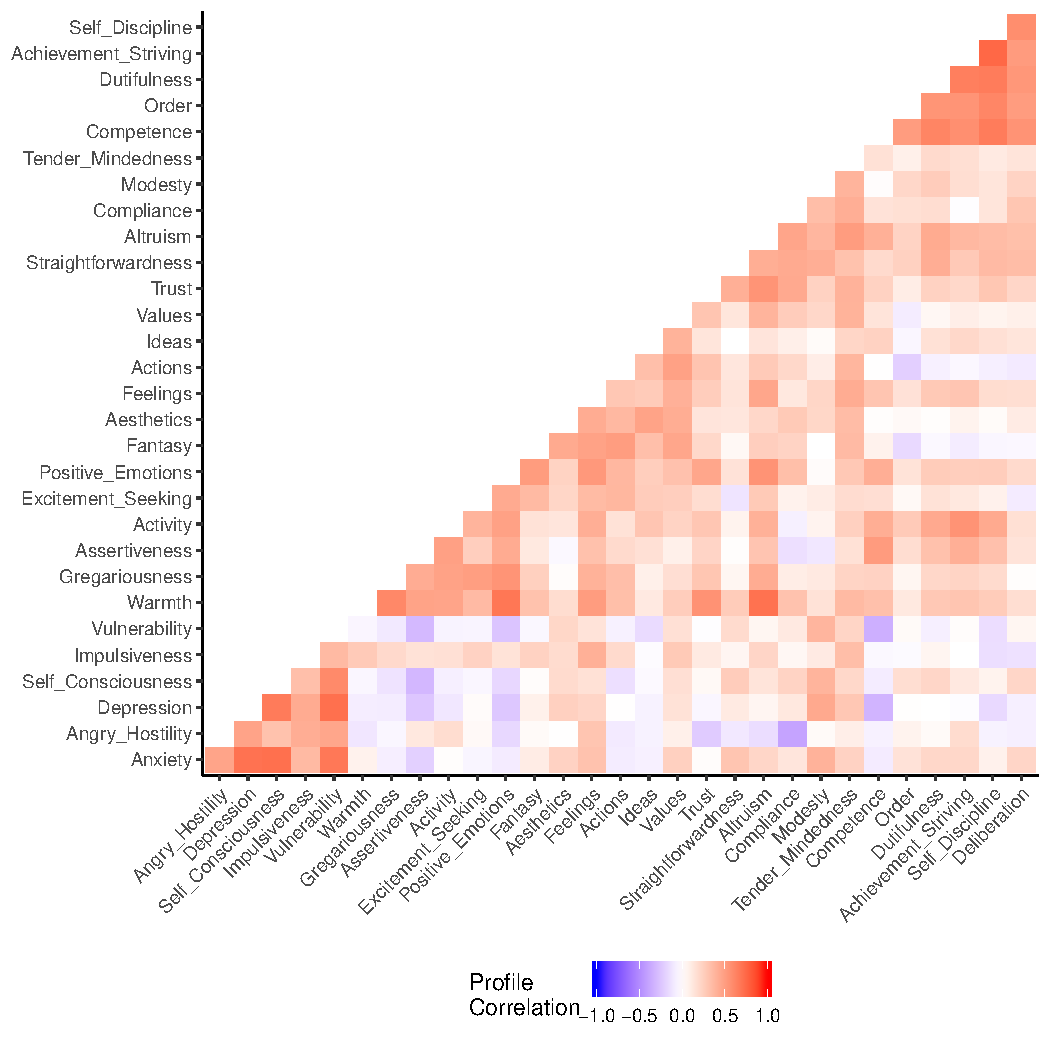
\includegraphics[width=\maxwidth]{figure/unnamed-chunk-5-1} 

\end{knitrout}

There appear to be intercorrelations among the variables.  

\subsubsection{KMO}
\begin{knitrout}
\definecolor{shadecolor}{rgb}{0.969, 0.969, 0.969}\color{fgcolor}\begin{kframe}
\begin{alltt}
\hlstd{(KMO1} \hlkwb{<-} \hlkwd{KMO}\hlstd{(r))}
\end{alltt}
\begin{verbatim}
## Kaiser-Meyer-Olkin factor adequacy
## Call: KMO(r = r)
## Overall MSA =  0.86
## MSA for each item = 
##              Anxiety      Angry_Hostility           Depression 
##                 0.85                 0.74                 0.81 
##   Self_Consciousness        Impulsiveness        Vulnerability 
##                 0.89                 0.87                 0.85 
##               Warmth       Gregariousness        Assertiveness 
##                 0.88                 0.88                 0.87 
##             Activity   Excitement_Seeking    Positive_Emotions 
##                 0.88                 0.85                 0.89 
##              Fantasy           Aesthetics             Feelings 
##                 0.84                 0.80                 0.90 
##              Actions                Ideas               Values 
##                 0.85                 0.78                 0.84 
##                Trust  Straightforwardness             Altruism 
##                 0.90                 0.80                 0.91 
##           Compliance              Modesty    Tender_Mindedness 
##                 0.79                 0.85                 0.90 
##           Competence                Order          Dutifulness 
##                 0.89                 0.88                 0.90 
## Achievement_Striving      Self_Discipline         Deliberation 
##                 0.89                 0.87                 0.86
\end{verbatim}
\end{kframe}
\end{knitrout}

The MSA for each item range from 1 to 1, with a mean of 1, indicating strong evidence for using a data reduction technique. 

\subsubsection{Bartlett's Test}
\begin{knitrout}
\definecolor{shadecolor}{rgb}{0.969, 0.969, 0.969}\color{fgcolor}\begin{kframe}
\begin{alltt}
\hlstd{(CB_1} \hlkwb{<-} \hlkwd{cortest.bartlett}\hlstd{(}\hlkwc{R}\hlstd{=r,}\hlkwc{n}\hlstd{=}\hlkwd{nrow}\hlstd{(dat)))}
\end{alltt}
\begin{verbatim}
## $chisq
## [1] 3707.648
## 
## $p.value
## [1] 0
## 
## $df
## [1] 435
\end{verbatim}
\end{kframe}
\end{knitrout}

In addition, the $\chi^2$ value of the Bartlett test ($\chi^2$(435) = 3707.65), which indicates that the correlation matrix departs significantly from from an identity matrix (independence among indicators).  



\subsection{How Many Factors?}
Now that we have seen evidence suggesting that we should conduct a CFA or PCA, we need to determine how many factors we should extract. 
\subsubsection{Parallel Analysis (Scree Test)}
\begin{knitrout}
\definecolor{shadecolor}{rgb}{0.969, 0.969, 0.969}\color{fgcolor}\begin{kframe}
\begin{alltt}
\hlkwd{par}\hlstd{(}\hlkwc{mfrow}\hlstd{=}\hlkwd{c}\hlstd{(}\hlnum{1}\hlstd{,}\hlnum{2}\hlstd{))}
\hlstd{scree_1} \hlkwb{<-} \hlkwd{fa.parallel}\hlstd{(dat} \hlopt \hlkwd{select}\hlstd{(}\hlopt{-}\hlstd{ID),} \hlkwc{fa}\hlstd{=}\hlstr{"both"}\hlstd{)}
\end{alltt}
\begin{verbatim}
## Parallel analysis suggests that the number of factors =  5  and the number of components =  5
\end{verbatim}
\begin{alltt}
\hlstd{scree_2} \hlkwb{<-} \hlkwd{fa.parallel}\hlstd{(r,} \hlkwc{fa} \hlstd{=} \hlstr{"both"}\hlstd{,} \hlkwc{n.obs} \hlstd{=} \hlkwd{nrow}\hlstd{(dat))}
\end{alltt}
\end{kframe}
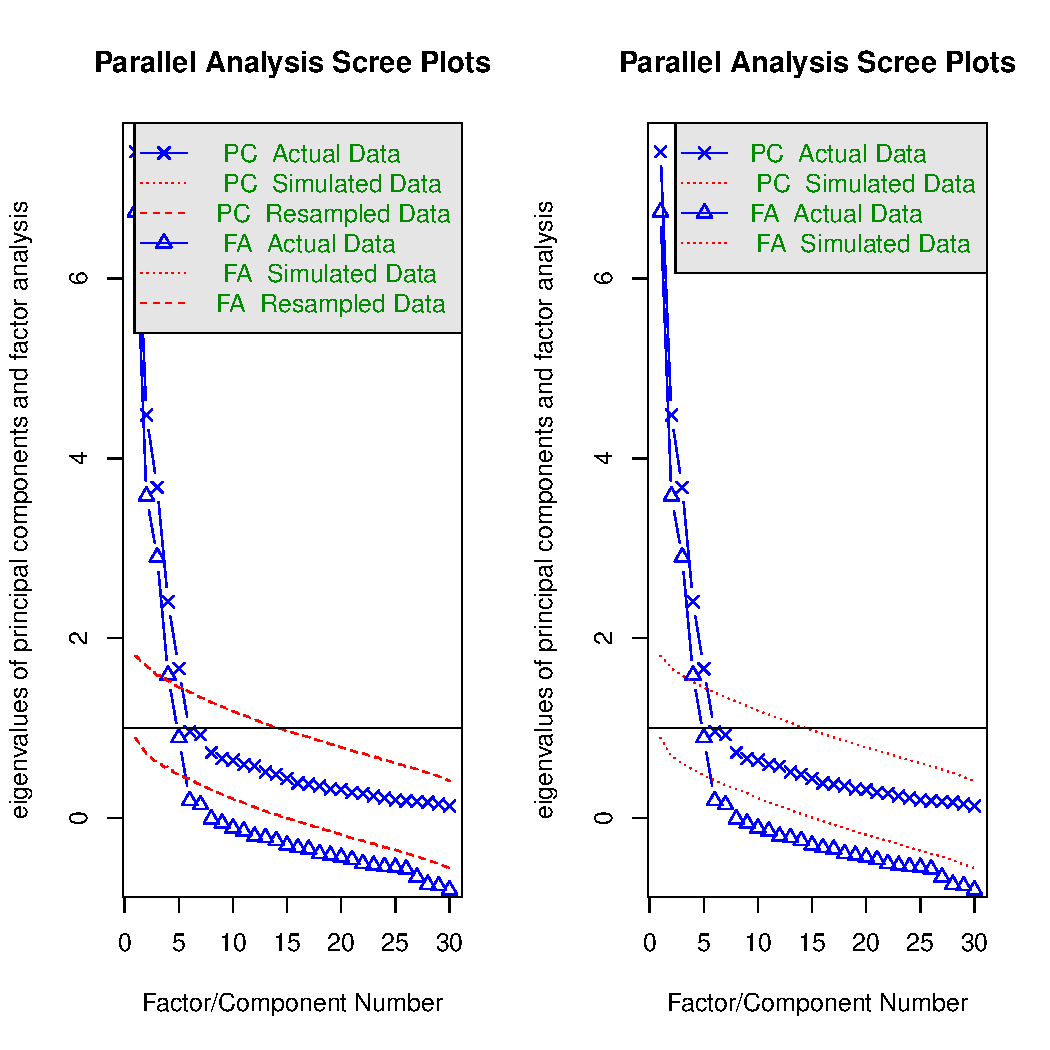
\includegraphics[width=\maxwidth]{figure/unnamed-chunk-8-1} 
\begin{kframe}\begin{verbatim}
## Parallel analysis suggests that the number of factors =  5  and the number of components =  5
\end{verbatim}
\end{kframe}
\end{knitrout}

Parallel analysis suggests 5 principal components and 5 factors. 

\subsubsection{VSS}
\begin{knitrout}
\definecolor{shadecolor}{rgb}{0.969, 0.969, 0.969}\color{fgcolor}\begin{kframe}
\begin{alltt}
\hlkwd{par}\hlstd{(}\hlkwc{mfrow} \hlstd{=} \hlkwd{c}\hlstd{(}\hlnum{1}\hlstd{,}\hlnum{1}\hlstd{))}
\hlstd{vss_1} \hlkwb{<-} \hlkwd{vss}\hlstd{(dat} \hlopt \hlkwd{select}\hlstd{(}\hlopt{-}\hlstd{ID),} \hlkwc{n} \hlstd{=} \hlnum{25}\hlstd{,} \hlkwc{rotate} \hlstd{=} \hlstr{"none"}\hlstd{,} \hlkwc{fm} \hlstd{=} \hlstr{"pc"}\hlstd{)}
\end{alltt}
\end{kframe}
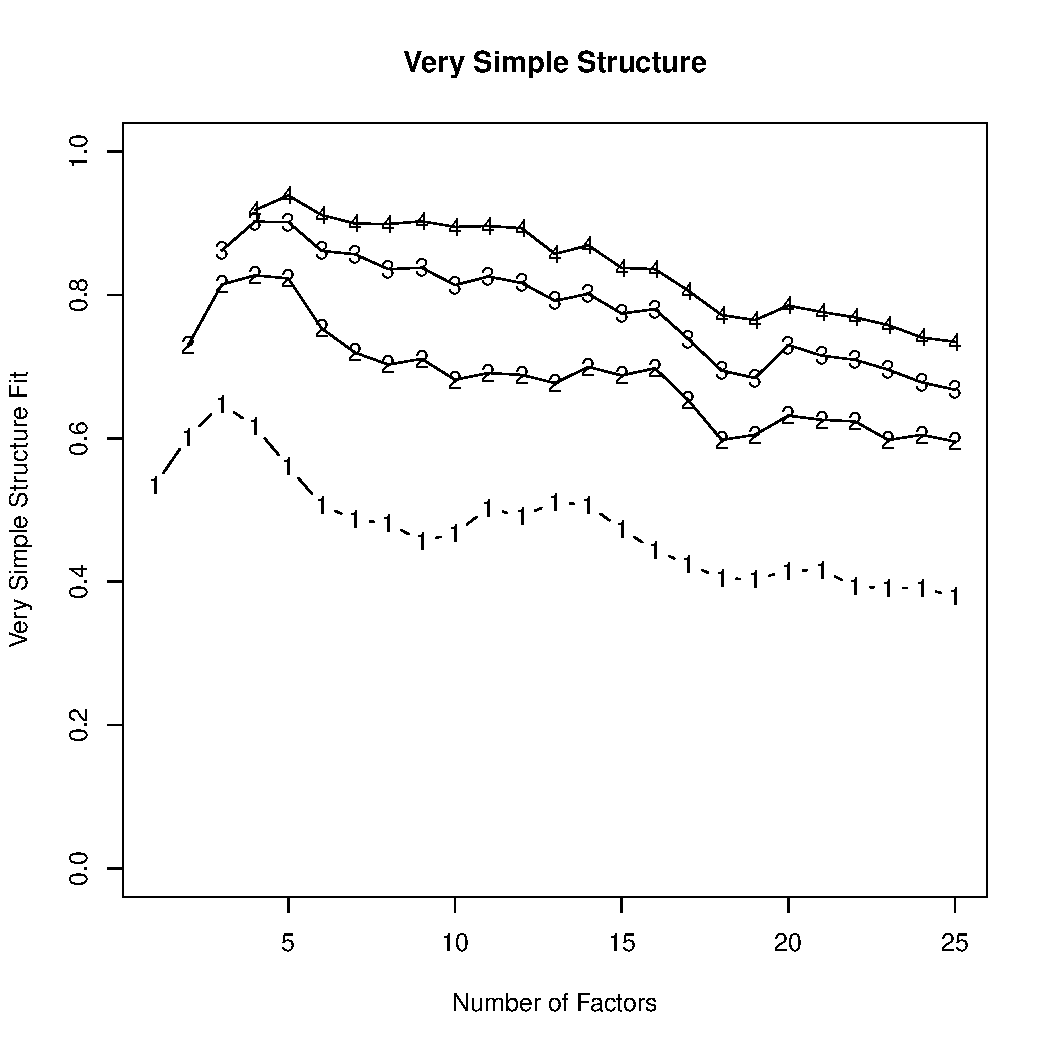
\includegraphics[width=\maxwidth]{figure/unnamed-chunk-9-1} 

\end{knitrout}

VSS also suggests 5 factors.  

\subsection{Exploratory Factor Analysis}
\begin{knitrout}
\definecolor{shadecolor}{rgb}{0.969, 0.969, 0.969}\color{fgcolor}\begin{kframe}
\begin{alltt}
\hlstd{fa_1} \hlkwb{<-} \hlkwd{fa}\hlstd{(dat} \hlopt \hlkwd{select}\hlstd{(}\hlopt{-}\hlstd{ID),} \hlkwc{nfactors} \hlstd{=} \hlnum{5}\hlstd{,} \hlkwc{rotate} \hlstd{=} \hlstr{"none"}\hlstd{,} \hlkwc{scores} \hlstd{= T)}
\hlstd{fa_2} \hlkwb{<-} \hlkwd{fa}\hlstd{(dat} \hlopt \hlkwd{select}\hlstd{(}\hlopt{-}\hlstd{ID),} \hlkwc{nfactors} \hlstd{=} \hlnum{5}\hlstd{,} \hlkwc{rotate} \hlstd{=} \hlstr{"varimax"}\hlstd{,} \hlkwc{scores} \hlstd{= T)}
\hlstd{fa_3} \hlkwb{<-} \hlkwd{fa}\hlstd{(dat} \hlopt \hlkwd{select}\hlstd{(}\hlopt{-}\hlstd{ID),} \hlkwc{nfactors} \hlstd{=} \hlnum{5}\hlstd{,} \hlkwc{rotate} \hlstd{=} \hlstr{"oblimin"}\hlstd{,} \hlkwc{scores} \hlstd{= T)}

\hlstd{scores_1} \hlkwb{<-} \hlstd{fa_1}\hlopt{$}\hlstd{scores}
\hlstd{scores_2} \hlkwb{<-} \hlstd{fa_2}\hlopt{$}\hlstd{scores}
\hlstd{scores_3} \hlkwb{<-} \hlstd{fa_3}\hlopt{$}\hlstd{scores}

\hlcom{# unrotated}
\hlkwd{cor}\hlstd{(scores_1)} \hlopt \hlkwd{round}\hlstd{(.,} \hlnum{2}\hlstd{)}
\end{alltt}
\begin{verbatim}
##       MR1  MR2  MR3  MR4   MR5
## MR1  1.00 0.00 0.01 0.00 -0.01
## MR2  0.00 1.00 0.00 0.01  0.00
## MR3  0.01 0.00 1.00 0.01  0.02
## MR4  0.00 0.01 0.01 1.00  0.00
## MR5 -0.01 0.00 0.02 0.00  1.00
\end{verbatim}
\begin{alltt}
\hlcom{# varimax rotation}
\hlkwd{cor}\hlstd{(scores_2)} \hlopt \hlkwd{round}\hlstd{(.,} \hlnum{2}\hlstd{)}
\end{alltt}
\begin{verbatim}
##       MR3   MR2   MR1   MR5  MR4
## MR3  1.00  0.00  0.04 -0.01 0.02
## MR2  0.00  1.00 -0.01  0.02 0.01
## MR1  0.04 -0.01  1.00  0.08 0.02
## MR5 -0.01  0.02  0.08  1.00 0.04
## MR4  0.02  0.01  0.02  0.04 1.00
\end{verbatim}
\begin{alltt}
\hlcom{# oblimin rotation}
\hlkwd{cor}\hlstd{(scores_3)} \hlopt \hlkwd{round}\hlstd{(.,} \hlnum{2}\hlstd{)}
\end{alltt}
\begin{verbatim}
##      MR3  MR2  MR1  MR5  MR4
## MR3 1.00 0.02 0.32 0.11 0.09
## MR2 0.02 1.00 0.00 0.11 0.04
## MR1 0.32 0.00 1.00 0.46 0.07
## MR5 0.11 0.11 0.46 1.00 0.11
## MR4 0.09 0.04 0.07 0.11 1.00
\end{verbatim}
\end{kframe}
\end{knitrout}


The two models fit the data relatively well ($RMSEA_{unrotated} = 0.0677843$, $RMSEA_{varimax} = 0.0677843$, $RMSEA_{oblimin} = 0.0677843$, $TLI_{unrotated} = 0.8938015$; $TLI_{varimax} = 0.8938015$; $TLI_{oblimin} = 0.8938015$). 

But we aren't just concerned with model fit. We are also generally interested in naming the factors. 

There's no way for me to pretend I don't have expectations for how the data should come out. So let's look at the rotated and unrotated solutions and see if we managed to recover the Big 5. 
\begin{kframe}
\begin{alltt}
\hlstd{fa_1}\hlopt{$}\hlstd{Structure} \hlopt \hlstd{unclass} \hlopt
  \hlstd{data.frame} \hlopt
  \hlkwd{mutate}\hlstd{(}\hlkwc{Facet} \hlstd{=} \hlkwd{rownames}\hlstd{(.))} \hlopt
  \hlkwd{full_join}\hlstd{(source)} \hlopt
  \hlkwd{select}\hlstd{(Factor, Facet, MR1, MR2, MR3, MR4, MR5)} \hlopt
  \hlkwd{mutate_at}\hlstd{(}\hlkwd{vars}\hlstd{(MR1}\hlopt{:}\hlstd{MR5),} \hlkwd{funs}\hlstd{(}\hlkwd{round}\hlstd{(.,} \hlnum{2}\hlstd{)))} \hlopt
  \hlkwd{mutate_at}\hlstd{(}\hlkwd{vars}\hlstd{(MR1}\hlopt{:}\hlstd{MR5),} \hlkwd{funs}\hlstd{(}\hlkwd{cell_spec}\hlstd{(.,} \hlstr{"latex"}\hlstd{,}
        \hlkwc{background} \hlstd{=} \hlkwd{ifelse}\hlstd{((.)} \hlopt{>} \hlnum{.5}\hlstd{,} \hlstr{"yellow"}\hlstd{,} \hlstr{"white"}\hlstd{))))} \hlopt
  \hlkwd{mutate}\hlstd{(}\hlkwc{Facet} \hlstd{=} \hlkwd{str_remove_all}\hlstd{(Facet,} \hlstr{"_"}\hlstd{))} \hlopt
  \hlkwd{kable}\hlstd{(.,} \hlstr{"latex"}\hlstd{,} \hlkwc{escape} \hlstd{= F,} \hlkwc{booktabs} \hlstd{= T,}
        \hlkwc{caption} \hlstd{=} \hlstr{"Unrotated Solution"}\hlstd{)} \hlopt
  \hlkwd{kable_styling}\hlstd{(}\hlkwc{full_width} \hlstd{= F)}
\end{alltt}
\end{kframe}\begin{table}

\caption{\label{tab:unnamed-chunk-11}Unrotated Solution}
\centering
\begin{tabular}[t]{lllllll}
\toprule
Factor & Facet & MR1 & MR2 & MR3 & MR4 & MR5\\
\midrule
Neuroticism & Anxiety & \cellcolor{white}{0.26} & \cellcolor{yellow}{0.78} & \cellcolor{white}{0.25} & \cellcolor{white}{0.09} & \cellcolor{white}{0}\\
Neuroticism & AngryHostility & \cellcolor{white}{0.03} & \cellcolor{white}{0.47} & \cellcolor{white}{0.12} & \cellcolor{yellow}{0.69} & \cellcolor{white}{0.02}\\
Neuroticism & Depression & \cellcolor{white}{0.08} & \cellcolor{yellow}{0.87} & \cellcolor{white}{0.05} & \cellcolor{white}{0.12} & \cellcolor{white}{-0.05}\\
Neuroticism & SelfConsciousness & \cellcolor{white}{0.17} & \cellcolor{yellow}{0.72} & \cellcolor{white}{0.28} & \cellcolor{white}{-0.04} & \cellcolor{white}{0.03}\\
Neuroticism & Impulsiveness & \cellcolor{white}{0.29} & \cellcolor{white}{0.43} & \cellcolor{white}{-0.22} & \cellcolor{white}{0.31} & \cellcolor{white}{-0.18}\\
\addlinespace
Neuroticism & Vulnerability & \cellcolor{white}{0.05} & \cellcolor{yellow}{0.81} & \cellcolor{white}{0.12} & \cellcolor{white}{0.07} & \cellcolor{white}{-0.11}\\
Extraversion & Warmth & \cellcolor{yellow}{0.73} & \cellcolor{white}{-0.14} & \cellcolor{white}{-0.24} & \cellcolor{white}{-0.01} & \cellcolor{white}{-0.38}\\
Extraversion & Gregariousness & \cellcolor{yellow}{0.53} & \cellcolor{white}{-0.2} & \cellcolor{white}{-0.27} & \cellcolor{white}{0.19} & \cellcolor{white}{-0.34}\\
Extraversion & Assertiveness & \cellcolor{white}{0.47} & \cellcolor{white}{-0.42} & \cellcolor{white}{-0.04} & \cellcolor{white}{0.38} & \cellcolor{white}{-0.12}\\
Extraversion & Activity & \cellcolor{yellow}{0.62} & \cellcolor{white}{-0.21} & \cellcolor{white}{0.02} & \cellcolor{white}{0.38} & \cellcolor{white}{-0.02}\\
\addlinespace
Extraversion & ExcitementSeeking & \cellcolor{white}{0.42} & \cellcolor{white}{-0.07} & \cellcolor{white}{-0.35} & \cellcolor{white}{0.22} & \cellcolor{white}{-0.01}\\
Extraversion & PositiveEmotions & \cellcolor{yellow}{0.7} & \cellcolor{white}{-0.3} & \cellcolor{white}{-0.32} & \cellcolor{white}{-0.01} & \cellcolor{white}{-0.08}\\
Openness & Fantasy & \cellcolor{white}{0.41} & \cellcolor{white}{0.1} & \cellcolor{white}{-0.55} & \cellcolor{white}{0} & \cellcolor{white}{0.24}\\
Openness & Aesthetics & \cellcolor{white}{0.37} & \cellcolor{white}{0.3} & \cellcolor{white}{-0.3} & \cellcolor{white}{-0.1} & \cellcolor{white}{0.46}\\
Openness & Feelings & \cellcolor{yellow}{0.66} & \cellcolor{white}{0.19} & \cellcolor{white}{-0.22} & \cellcolor{white}{0.27} & \cellcolor{white}{0.07}\\
\addlinespace
Openness & Actions & \cellcolor{white}{0.38} & \cellcolor{white}{0.01} & \cellcolor{white}{-0.57} & \cellcolor{white}{-0.09} & \cellcolor{white}{0.12}\\
Openness & Ideas & \cellcolor{white}{0.35} & \cellcolor{white}{-0.09} & \cellcolor{white}{-0.23} & \cellcolor{white}{0.02} & \cellcolor{yellow}{0.57}\\
Openness & Values & \cellcolor{white}{0.47} & \cellcolor{white}{0.24} & \cellcolor{white}{-0.35} & \cellcolor{white}{-0.05} & \cellcolor{white}{0.27}\\
Agreeableness & Trust & \cellcolor{yellow}{0.57} & \cellcolor{white}{-0.06} & \cellcolor{white}{-0.12} & \cellcolor{white}{-0.31} & \cellcolor{white}{-0.2}\\
Agreeableness & Straightforwardness & \cellcolor{white}{0.43} & \cellcolor{white}{0.19} & \cellcolor{white}{0.26} & \cellcolor{white}{-0.4} & \cellcolor{white}{-0.1}\\
\addlinespace
Agreeableness & Altruism & \cellcolor{yellow}{0.78} & \cellcolor{white}{0.03} & \cellcolor{white}{-0.04} & \cellcolor{white}{-0.21} & \cellcolor{white}{-0.24}\\
Agreeableness & Compliance & \cellcolor{white}{0.42} & \cellcolor{white}{0.17} & \cellcolor{white}{-0.06} & \cellcolor{white}{-0.67} & \cellcolor{white}{-0.05}\\
Agreeableness & Modesty & \cellcolor{white}{0.36} & \cellcolor{white}{0.43} & \cellcolor{white}{0.15} & \cellcolor{white}{-0.24} & \cellcolor{white}{-0.09}\\
Agreeableness & TenderMindedness & \cellcolor{yellow}{0.55} & \cellcolor{white}{0.29} & \cellcolor{white}{-0.19} & \cellcolor{white}{-0.13} & \cellcolor{white}{0}\\
Conscientiousness & Competence & \cellcolor{yellow}{0.6} & \cellcolor{white}{-0.42} & \cellcolor{white}{0.35} & \cellcolor{white}{0.07} & \cellcolor{white}{0.15}\\
\addlinespace
Conscientiousness & Order & \cellcolor{white}{0.39} & \cellcolor{white}{-0.08} & \cellcolor{yellow}{0.59} & \cellcolor{white}{0.03} & \cellcolor{white}{0.05}\\
Conscientiousness & Dutifulness & \cellcolor{yellow}{0.61} & \cellcolor{white}{-0.11} & \cellcolor{yellow}{0.52} & \cellcolor{white}{0.04} & \cellcolor{white}{0.03}\\
Conscientiousness & AchievementStriving & \cellcolor{yellow}{0.6} & \cellcolor{white}{-0.14} & \cellcolor{yellow}{0.52} & \cellcolor{white}{0.25} & \cellcolor{white}{0.11}\\
Conscientiousness & SelfDiscipline & \cellcolor{yellow}{0.57} & \cellcolor{white}{-0.28} & \cellcolor{yellow}{0.57} & \cellcolor{white}{0} & \cellcolor{white}{0.14}\\
Conscientiousness & Deliberation & \cellcolor{white}{0.46} & \cellcolor{white}{-0.06} & \cellcolor{yellow}{0.52} & \cellcolor{white}{-0.2} & \cellcolor{white}{0.19}\\
\bottomrule
\end{tabular}
\end{table}

\begin{kframe}\begin{alltt}
\hlstd{fa_2}\hlopt{$}\hlstd{Structure} \hlopt \hlstd{unclass} \hlopt
  \hlstd{data.frame} \hlopt
  \hlkwd{mutate}\hlstd{(}\hlkwc{Facet} \hlstd{=} \hlkwd{rownames}\hlstd{(.))} \hlopt
  \hlkwd{full_join}\hlstd{(source)} \hlopt
  \hlkwd{select}\hlstd{(Factor, Facet, MR1, MR2, MR3, MR4, MR5)} \hlopt
  \hlkwd{mutate_at}\hlstd{(}\hlkwd{vars}\hlstd{(MR1}\hlopt{:}\hlstd{MR5),} \hlkwd{funs}\hlstd{(}\hlkwd{round}\hlstd{(.,} \hlnum{2}\hlstd{)))} \hlopt
  \hlkwd{mutate_at}\hlstd{(}\hlkwd{vars}\hlstd{(MR1}\hlopt{:}\hlstd{MR5),} \hlkwd{funs}\hlstd{(}\hlkwd{cell_spec}\hlstd{(.,} \hlstr{"latex"}\hlstd{,}
        \hlkwc{background} \hlstd{=} \hlkwd{ifelse}\hlstd{(}\hlkwd{abs}\hlstd{(.)} \hlopt{>} \hlnum{.5}\hlstd{,} \hlstr{"yellow"}\hlstd{,} \hlstr{"white"}\hlstd{))))} \hlopt
  \hlkwd{mutate}\hlstd{(}\hlkwc{Facet} \hlstd{=} \hlkwd{str_remove_all}\hlstd{(Facet,} \hlstr{"_"}\hlstd{))} \hlopt
  \hlkwd{kable}\hlstd{(.,} \hlstr{"latex"}\hlstd{,} \hlkwc{escape} \hlstd{= F,} \hlkwc{booktabs} \hlstd{= T,}
        \hlkwc{caption} \hlstd{=} \hlstr{"Varimax Rotated Solution"}\hlstd{)} \hlopt
  \hlkwd{kable_styling}\hlstd{(}\hlkwc{full_width} \hlstd{= F)}
\end{alltt}
\end{kframe}\begin{table}

\caption{\label{tab:unnamed-chunk-11}Varimax Rotated Solution}
\centering
\begin{tabular}[t]{lllllll}
\toprule
Factor & Facet & MR1 & MR2 & MR3 & MR4 & MR5\\
\midrule
Neuroticism & Anxiety & \cellcolor{white}{-0.05} & \cellcolor{yellow}{0.84} & \cellcolor{white}{0.16} & \cellcolor{white}{0.1} & \cellcolor{white}{0.07}\\
Neuroticism & AngryHostility & \cellcolor{white}{0.14} & \cellcolor{yellow}{0.62} & \cellcolor{white}{0.07} & \cellcolor{yellow}{-0.55} & \cellcolor{white}{0}\\
Neuroticism & Depression & \cellcolor{white}{-0.07} & \cellcolor{yellow}{0.86} & \cellcolor{white}{-0.13} & \cellcolor{white}{0.03} & \cellcolor{white}{0.08}\\
Neuroticism & SelfConsciousness & \cellcolor{white}{-0.18} & \cellcolor{yellow}{0.74} & \cellcolor{white}{0.14} & \cellcolor{white}{0.17} & \cellcolor{white}{0.05}\\
Neuroticism & Impulsiveness & \cellcolor{white}{0.4} & \cellcolor{white}{0.5} & \cellcolor{white}{-0.12} & \cellcolor{white}{-0.07} & \cellcolor{white}{0.13}\\
\addlinespace
Neuroticism & Vulnerability & \cellcolor{white}{-0.09} & \cellcolor{yellow}{0.82} & \cellcolor{white}{-0.1} & \cellcolor{white}{0.08} & \cellcolor{white}{-0.02}\\
Extraversion & Warmth & \cellcolor{yellow}{0.77} & \cellcolor{white}{0} & \cellcolor{white}{0.15} & \cellcolor{white}{0.37} & \cellcolor{white}{0.1}\\
Extraversion & Gregariousness & \cellcolor{yellow}{0.72} & \cellcolor{white}{-0.06} & \cellcolor{white}{0.07} & \cellcolor{white}{0.09} & \cellcolor{white}{0.05}\\
Extraversion & Assertiveness & \cellcolor{yellow}{0.6} & \cellcolor{white}{-0.22} & \cellcolor{white}{0.34} & \cellcolor{white}{-0.18} & \cellcolor{white}{0.04}\\
Extraversion & Activity & \cellcolor{yellow}{0.57} & \cellcolor{white}{0} & \cellcolor{white}{0.44} & \cellcolor{white}{-0.13} & \cellcolor{white}{0.17}\\
\addlinespace
Extraversion & ExcitementSeeking & \cellcolor{white}{0.5} & \cellcolor{white}{-0.01} & \cellcolor{white}{0.01} & \cellcolor{white}{-0.04} & \cellcolor{white}{0.31}\\
Extraversion & PositiveEmotions & \cellcolor{yellow}{0.65} & \cellcolor{white}{-0.21} & \cellcolor{white}{0.19} & \cellcolor{white}{0.25} & \cellcolor{white}{0.33}\\
Openness & Fantasy & \cellcolor{white}{0.32} & \cellcolor{white}{0.03} & \cellcolor{white}{-0.15} & \cellcolor{white}{0.1} & \cellcolor{yellow}{0.63}\\
Openness & Aesthetics & \cellcolor{white}{0.01} & \cellcolor{white}{0.21} & \cellcolor{white}{0.02} & \cellcolor{white}{0.14} & \cellcolor{yellow}{0.69}\\
Openness & Feelings & \cellcolor{yellow}{0.53} & \cellcolor{white}{0.3} & \cellcolor{white}{0.2} & \cellcolor{white}{0} & \cellcolor{white}{0.43}\\
\addlinespace
Openness & Actions & \cellcolor{white}{0.36} & \cellcolor{white}{-0.07} & \cellcolor{white}{-0.2} & \cellcolor{white}{0.19} & \cellcolor{yellow}{0.53}\\
Openness & Ideas & \cellcolor{white}{0.04} & \cellcolor{white}{-0.13} & \cellcolor{white}{0.19} & \cellcolor{white}{-0.05} & \cellcolor{yellow}{0.67}\\
Openness & Values & \cellcolor{white}{0.22} & \cellcolor{white}{0.19} & \cellcolor{white}{0} & \cellcolor{white}{0.17} & \cellcolor{yellow}{0.6}\\
Agreeableness & Trust & \cellcolor{white}{0.39} & \cellcolor{white}{-0.02} & \cellcolor{white}{0.15} & \cellcolor{yellow}{0.53} & \cellcolor{white}{0.14}\\
Agreeableness & Straightforwardness & \cellcolor{white}{0.03} & \cellcolor{white}{0.22} & \cellcolor{white}{0.32} & \cellcolor{yellow}{0.55} & \cellcolor{white}{0}\\
\addlinespace
Agreeableness & Altruism & \cellcolor{yellow}{0.53} & \cellcolor{white}{0.13} & \cellcolor{white}{0.3} & \cellcolor{yellow}{0.54} & \cellcolor{white}{0.16}\\
Agreeableness & Compliance & \cellcolor{white}{0.01} & \cellcolor{white}{0.07} & \cellcolor{white}{0.07} & \cellcolor{yellow}{0.78} & \cellcolor{white}{0.21}\\
Agreeableness & Modesty & \cellcolor{white}{0.03} & \cellcolor{white}{0.44} & \cellcolor{white}{0.16} & \cellcolor{white}{0.41} & \cellcolor{white}{0.07}\\
Agreeableness & TenderMindedness & \cellcolor{white}{0.31} & \cellcolor{white}{0.3} & \cellcolor{white}{0.08} & \cellcolor{white}{0.36} & \cellcolor{white}{0.36}\\
Conscientiousness & Competence & \cellcolor{white}{0.27} & \cellcolor{white}{-0.24} & \cellcolor{yellow}{0.74} & \cellcolor{white}{0.06} & \cellcolor{white}{0.12}\\
\addlinespace
Conscientiousness & Order & \cellcolor{white}{0.02} & \cellcolor{white}{0.1} & \cellcolor{yellow}{0.69} & \cellcolor{white}{0.09} & \cellcolor{white}{-0.11}\\
Conscientiousness & Dutifulness & \cellcolor{white}{0.2} & \cellcolor{white}{0.1} & \cellcolor{yellow}{0.76} & \cellcolor{white}{0.16} & \cellcolor{white}{-0.02}\\
Conscientiousness & AchievementStriving & \cellcolor{white}{0.24} & \cellcolor{white}{0.11} & \cellcolor{yellow}{0.81} & \cellcolor{white}{-0.05} & \cellcolor{white}{0.03}\\
Conscientiousness & SelfDiscipline & \cellcolor{white}{0.12} & \cellcolor{white}{-0.08} & \cellcolor{yellow}{0.84} & \cellcolor{white}{0.13} & \cellcolor{white}{0.01}\\
Conscientiousness & Deliberation & \cellcolor{white}{-0.08} & \cellcolor{white}{0.05} & \cellcolor{yellow}{0.68} & \cellcolor{white}{0.28} & \cellcolor{white}{0.07}\\
\bottomrule
\end{tabular}
\end{table}

\begin{kframe}\begin{alltt}
\hlstd{fa_3}\hlopt{$}\hlstd{Structure} \hlopt \hlstd{unclass} \hlopt
  \hlstd{data.frame} \hlopt
  \hlkwd{mutate}\hlstd{(}\hlkwc{Facet} \hlstd{=} \hlkwd{rownames}\hlstd{(.))} \hlopt
  \hlkwd{full_join}\hlstd{(source)} \hlopt
  \hlkwd{select}\hlstd{(Factor, Facet, MR1, MR2, MR3, MR4, MR5)} \hlopt
  \hlkwd{mutate_at}\hlstd{(}\hlkwd{vars}\hlstd{(MR1}\hlopt{:}\hlstd{MR5),} \hlkwd{funs}\hlstd{(}\hlkwd{round}\hlstd{(.,} \hlnum{2}\hlstd{)))} \hlopt
  \hlkwd{mutate_at}\hlstd{(}\hlkwd{vars}\hlstd{(MR1}\hlopt{:}\hlstd{MR5),} \hlkwd{funs}\hlstd{(}\hlkwd{cell_spec}\hlstd{(.,} \hlstr{"latex"}\hlstd{,}
        \hlkwc{background} \hlstd{=} \hlkwd{ifelse}\hlstd{(}\hlkwd{abs}\hlstd{(.)} \hlopt{>} \hlnum{.5}\hlstd{,} \hlstr{"yellow"}\hlstd{,} \hlstr{"white"}\hlstd{))))} \hlopt
  \hlkwd{mutate}\hlstd{(}\hlkwc{Facet} \hlstd{=} \hlkwd{str_remove_all}\hlstd{(Facet,} \hlstr{"_"}\hlstd{))} \hlopt
  \hlkwd{kable}\hlstd{(.,} \hlstr{"latex"}\hlstd{,} \hlkwc{escape} \hlstd{= F,} \hlkwc{booktabs} \hlstd{= T,}
        \hlkwc{caption} \hlstd{=} \hlstr{"Oblimin Rotated Solution"}\hlstd{)} \hlopt
  \hlkwd{kable_styling}\hlstd{(}\hlkwc{full_width} \hlstd{= F)}
\end{alltt}
\end{kframe}\begin{table}

\caption{\label{tab:unnamed-chunk-11}Oblimin Rotated Solution}
\centering
\begin{tabular}[t]{lllllll}
\toprule
Factor & Facet & MR1 & MR2 & MR3 & MR4 & MR5\\
\midrule
Neuroticism & Anxiety & \cellcolor{white}{0.02} & \cellcolor{yellow}{0.85} & \cellcolor{white}{0.16} & \cellcolor{white}{0.05} & \cellcolor{white}{0.12}\\
Neuroticism & AngryHostility & \cellcolor{white}{0.01} & \cellcolor{yellow}{0.55} & \cellcolor{white}{0.04} & \cellcolor{yellow}{-0.61} & \cellcolor{white}{0.02}\\
Neuroticism & Depression & \cellcolor{white}{-0.05} & \cellcolor{yellow}{0.87} & \cellcolor{white}{-0.12} & \cellcolor{white}{-0.01} & \cellcolor{white}{0.1}\\
Neuroticism & SelfConsciousness & \cellcolor{white}{-0.08} & \cellcolor{yellow}{0.77} & \cellcolor{white}{0.14} & \cellcolor{white}{0.16} & \cellcolor{white}{0.06}\\
Neuroticism & Impulsiveness & \cellcolor{white}{0.37} & \cellcolor{white}{0.48} & \cellcolor{white}{-0.07} & \cellcolor{white}{-0.18} & \cellcolor{white}{0.24}\\
\addlinespace
Neuroticism & Vulnerability & \cellcolor{white}{-0.06} & \cellcolor{yellow}{0.82} & \cellcolor{white}{-0.1} & \cellcolor{white}{0.04} & \cellcolor{white}{0.01}\\
Extraversion & Warmth & \cellcolor{yellow}{0.86} & \cellcolor{white}{0} & \cellcolor{white}{0.3} & \cellcolor{white}{0.19} & \cellcolor{white}{0.32}\\
Extraversion & Gregariousness & \cellcolor{yellow}{0.72} & \cellcolor{white}{-0.09} & \cellcolor{white}{0.18} & \cellcolor{white}{-0.06} & \cellcolor{white}{0.23}\\
Extraversion & Assertiveness & \cellcolor{yellow}{0.57} & \cellcolor{white}{-0.26} & \cellcolor{white}{0.4} & \cellcolor{white}{-0.28} & \cellcolor{white}{0.17}\\
Extraversion & Activity & \cellcolor{yellow}{0.58} & \cellcolor{white}{-0.03} & \cellcolor{white}{0.5} & \cellcolor{white}{-0.24} & \cellcolor{white}{0.31}\\
\addlinespace
Extraversion & ExcitementSeeking & \cellcolor{white}{0.5} & \cellcolor{white}{-0.02} & \cellcolor{white}{0.08} & \cellcolor{white}{-0.13} & \cellcolor{white}{0.42}\\
Extraversion & PositiveEmotions & \cellcolor{yellow}{0.75} & \cellcolor{white}{-0.2} & \cellcolor{white}{0.31} & \cellcolor{white}{0.14} & \cellcolor{white}{0.5}\\
Openness & Fantasy & \cellcolor{white}{0.4} & \cellcolor{white}{0.05} & \cellcolor{white}{-0.08} & \cellcolor{white}{0.06} & \cellcolor{yellow}{0.69}\\
Openness & Aesthetics & \cellcolor{white}{0.14} & \cellcolor{white}{0.25} & \cellcolor{white}{0.05} & \cellcolor{white}{0.16} & \cellcolor{yellow}{0.69}\\
Openness & Feelings & \cellcolor{yellow}{0.59} & \cellcolor{white}{0.3} & \cellcolor{white}{0.28} & \cellcolor{white}{-0.11} & \cellcolor{yellow}{0.57}\\
\addlinespace
Openness & Actions & \cellcolor{white}{0.43} & \cellcolor{white}{-0.05} & \cellcolor{white}{-0.12} & \cellcolor{white}{0.14} & \cellcolor{yellow}{0.61}\\
Openness & Ideas & \cellcolor{white}{0.13} & \cellcolor{white}{-0.1} & \cellcolor{white}{0.2} & \cellcolor{white}{-0.01} & \cellcolor{yellow}{0.66}\\
Openness & Values & \cellcolor{white}{0.34} & \cellcolor{white}{0.22} & \cellcolor{white}{0.06} & \cellcolor{white}{0.14} & \cellcolor{yellow}{0.65}\\
Agreeableness & Trust & \cellcolor{yellow}{0.54} & \cellcolor{white}{0.01} & \cellcolor{white}{0.26} & \cellcolor{white}{0.44} & \cellcolor{white}{0.28}\\
Agreeableness & Straightforwardness & \cellcolor{white}{0.22} & \cellcolor{white}{0.27} & \cellcolor{white}{0.38} & \cellcolor{yellow}{0.52} & \cellcolor{white}{0.08}\\
\addlinespace
Agreeableness & Altruism & \cellcolor{yellow}{0.71} & \cellcolor{white}{0.16} & \cellcolor{white}{0.44} & \cellcolor{white}{0.41} & \cellcolor{white}{0.35}\\
Agreeableness & Compliance & \cellcolor{white}{0.25} & \cellcolor{white}{0.16} & \cellcolor{white}{0.15} & \cellcolor{yellow}{0.76} & \cellcolor{white}{0.28}\\
Agreeableness & Modesty & \cellcolor{white}{0.17} & \cellcolor{white}{0.48} & \cellcolor{white}{0.21} & \cellcolor{white}{0.37} & \cellcolor{white}{0.14}\\
Agreeableness & TenderMindedness & \cellcolor{white}{0.45} & \cellcolor{white}{0.33} & \cellcolor{white}{0.16} & \cellcolor{white}{0.28} & \cellcolor{white}{0.47}\\
Conscientiousness & Competence & \cellcolor{white}{0.37} & \cellcolor{white}{-0.23} & \cellcolor{yellow}{0.77} & \cellcolor{white}{0.03} & \cellcolor{white}{0.2}\\
\addlinespace
Conscientiousness & Order & \cellcolor{white}{0.11} & \cellcolor{white}{0.11} & \cellcolor{yellow}{0.69} & \cellcolor{white}{0.08} & \cellcolor{white}{-0.06}\\
Conscientiousness & Dutifulness & \cellcolor{white}{0.32} & \cellcolor{white}{0.11} & \cellcolor{yellow}{0.8} & \cellcolor{white}{0.11} & \cellcolor{white}{0.09}\\
Conscientiousness & AchievementStriving & \cellcolor{white}{0.31} & \cellcolor{white}{0.1} & \cellcolor{yellow}{0.83} & \cellcolor{white}{-0.1} & \cellcolor{white}{0.12}\\
Conscientiousness & SelfDiscipline & \cellcolor{white}{0.25} & \cellcolor{white}{-0.06} & \cellcolor{yellow}{0.86} & \cellcolor{white}{0.12} & \cellcolor{white}{0.08}\\
Conscientiousness & Deliberation & \cellcolor{white}{0.09} & \cellcolor{white}{0.09} & \cellcolor{yellow}{0.69} & \cellcolor{white}{0.29} & \cellcolor{white}{0.1}\\
\bottomrule
\end{tabular}
\end{table}



With the exception of the 2nd and 3rd factors, the unrotated solution doesn't resemble the expected solution. However, the indicators for each factor in the varimax rotated solution can clearly be identified as the Big 5 by content. Finally, in the oblimin rotated solution, we see that the factors can be fairly readily identified by content.  

Another fun test is the order of extraction, which is typically Extraversion, Agreeableness, Conscientiousness, Neuroticism, and Openness to Experience.  

In this case, the order of extraction for the rotated solutions appears to be Extraversion, Neuroticism, Conscientiousness, Agreeableness, Openness. 

\end{document}
